
\section{媒質に垂直入射した光の伝搬に関する偏光計算}
\label{sec:jones_and_U}
\subsection{Jones行列の導入}
単色平面波が一様媒質中を伝搬する状況を考える.伝搬方向を $\hat{\mathbf{k}}$ とし,電場は横波条件
\begin{equation}
\mathbf{E}\cdot\hat{\mathbf{k}}=0
\label{eq:transversality}
\end{equation}
を満たす.

単色平面波の横成分電場は
\begin{equation}
E_x(t)=A_x\cos(\omega t+\phi_x),\qquad
E_y(t)=A_y\cos(\omega t+\phi_y)
\label{eq:real_time_components}
\end{equation}
のように書ける.偏光楕円を決めるのは振幅比 $A_y/A_x$ と相対位相差
\begin{equation}
\delta=\phi_y-\phi_x
\label{eq:relative_phase}
\end{equation}
であり,「位相差 $\delta$」が偏光自由度に本質的に含まれる.これを複素表示(フェーザ)にすると
\begin{equation}
\tilde E_x=A_x e^{i\phi_x},\qquad \tilde E_y=A_y e^{i\phi_y}
\label{eq:phasors}
\end{equation}
となり,相対位相差は比 $\tilde E_y/\tilde E_x$ の偏角として自然に表現される.
このため Jonesベクトル
\begin{equation}
\mathbf{J}=
\begin{pmatrix}
\tilde E_x\\
\tilde E_y
\end{pmatrix}
\label{eq:J_phasor}
\end{equation}
は複素数成分を持つのが最も自然である.

\subsubsection*{直線偏光(linear polarization)のJones表現}
Jonesベクトルの複素成分は一般に振幅と位相を含むが,まず最も単純な場合として直線偏光を整理しておく.
直線偏光とは,2つの直交成分 $x$,$y$ の\emph{相対位相差}が
\begin{equation}
\delta \equiv \phi_y-\phi_x = 0 \ \ (\mathrm{mod}\ \pi)
\label{eq:linear_phase_condition}
\end{equation}
を満たす偏光状態である.すなわち2成分が同位相($\delta=0$)または反位相($\delta=\pi$)で振動するため,
電場ベクトルの先端は時間とともに一直線上を往復し,偏光楕円は退化して直線となる.

位相の基準(全体位相)を適当に選べば,直線偏光のJonesベクトルは実数2成分で表せる.
偏光方位角を $x$ 軸から $\alpha$ とすると,
\begin{equation}
\mathbf{J}_{\mathrm{lin}}(\alpha)
=
\begin{pmatrix}
\cos\alpha\\
\sin\alpha
\end{pmatrix}
\quad
\left(\text{全体位相因子 } e^{i\phi}\ \text{は物理的に無関係}\right)
\label{eq:linear_jones}
\end{equation}
と書ける.例えば $\alpha=0$ は $x$ 直線偏光,$\alpha=\pi/2$ は $y$ 直線偏光を与える.
ここで「全体位相(共通因子)$e^{i\phi}$ は観測される偏光状態を変えない」ことに注意する.
すなわち $\mathbf{J}$ と $e^{i\phi}\mathbf{J}$ は同じ偏光を表す(強度にも偏光楕円にも影響しない).

直線偏光が実数2成分で書けるのは,相対位相差が $0$ または $\pi$ に限定されているためであり,
相対位相差が一般値になるとJonesベクトルの複素性が本質となって楕円偏光(円偏光を含む)を表す.

右・左円偏光は
\begin{equation}
\mathbf{J}=\frac{1}{\sqrt2}\begin{pmatrix}1\\ i\end{pmatrix}
\qquad
(\text{あるいは } \frac{1}{\sqrt2}\begin{pmatrix}1\\ -i\end{pmatrix})
\label{eq:circular}
\end{equation}
のように虚数成分を本質的に含む.これは $y$ 成分が $x$ 成分より $\pi/2$ だけ進んでいることを意味する.
このように,
Jonesベクトルを実数2成分に限定すると,この相対位相 $\pm\pi/2$ を表現できず,
一般の楕円偏光を一つの枠組みで取り扱えない.
各種偏光状態を図~\ref{fig:appendix_1}に示す.

\begin{figure}[htb]
\centering
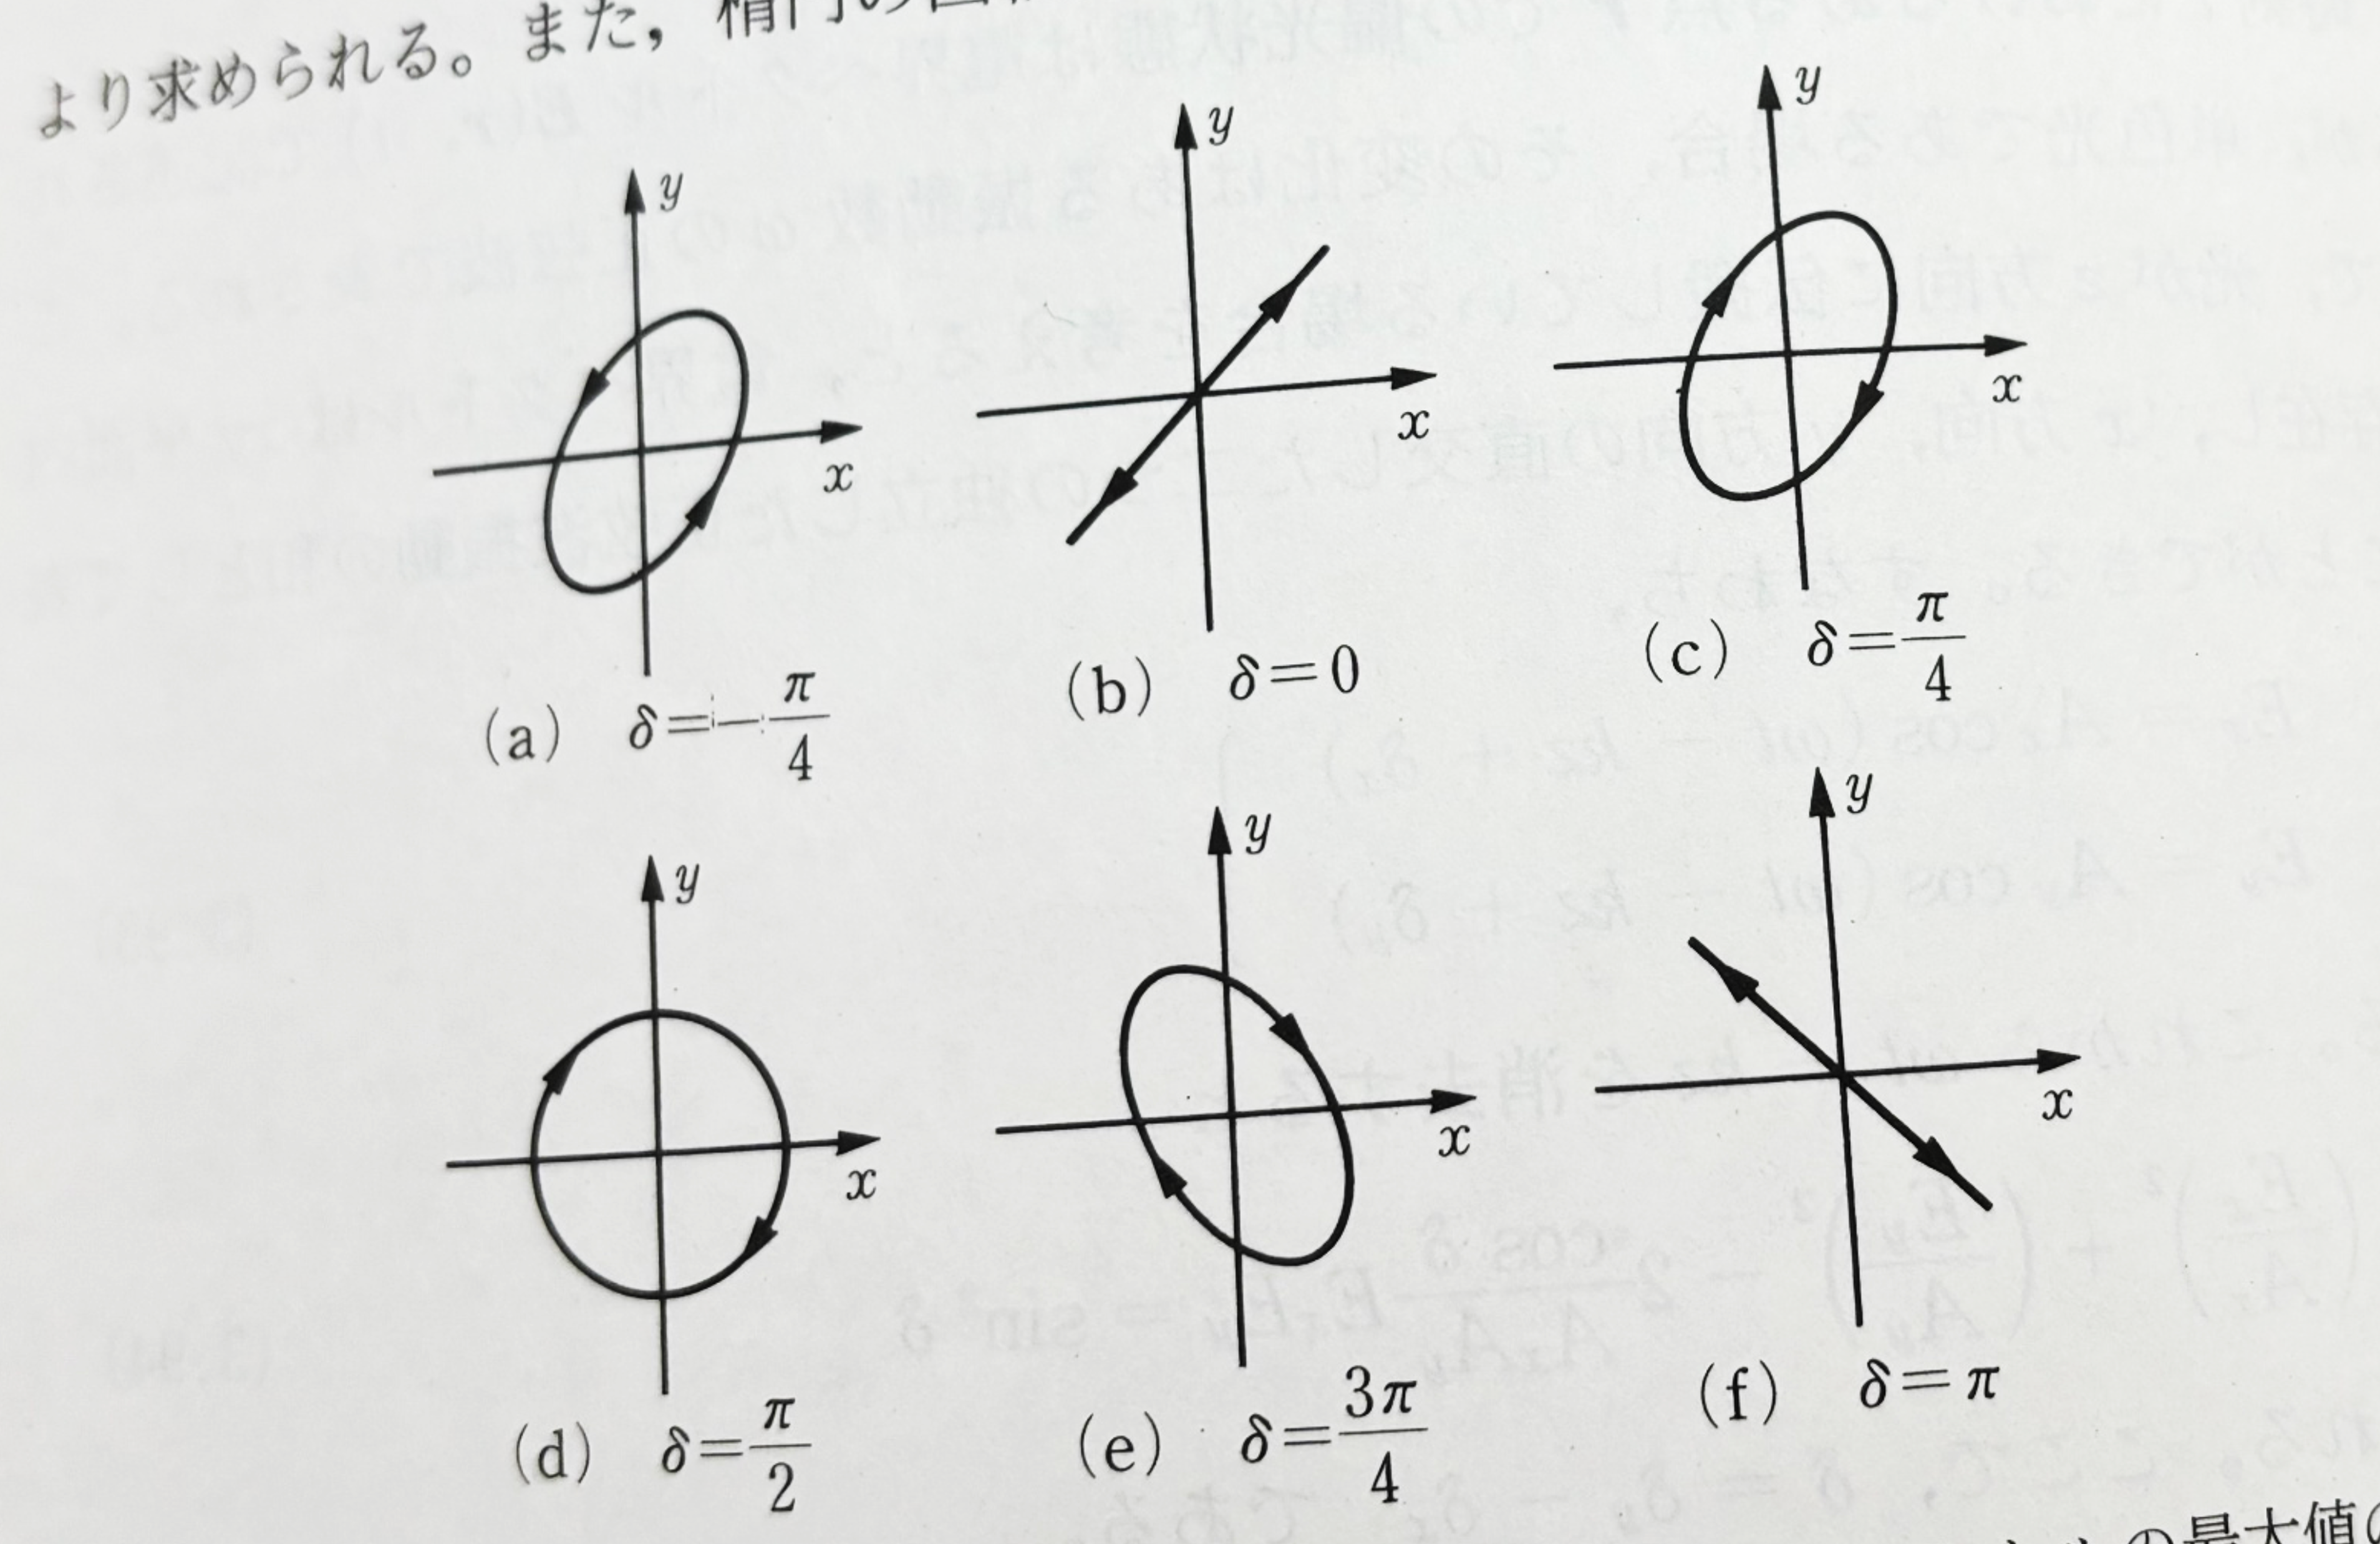
\includegraphics[width=0.92\linewidth]{appendix_1.png}
\caption{位相差$\delta$の違いによる偏光状態の変化.}
\label{fig:appendix_1}
\end{figure}


\subsubsection*{位相差(phase difference)とリタデーション(retardation)の定義}
一軸性媒質(単軸結晶や液晶補償板)では,電場は一般に互いに直交する2つの固有偏光(常光・異常光)に分解され,
それぞれ異なる屈折率で伝搬する.常光屈折率を $n_o$,異常光屈折率を $n_e$,板厚を $d$,真空波長を $\lambda$
とすると,両成分の光路差(optical path difference; OPD)は
\begin{equation}
\Delta L = (n_e-n_o)\,d \equiv \Delta n\,d
\label{eq:OPD}
\end{equation}
で与えられる.ここで $\Delta n=n_e-n_o$ を複屈折(birefringence)と呼ぶ.

\emph{リタデーション(retardation)}はこの光路差を長さとして表した量であり,文献により
$R=\Delta n\,d$(単位:長さ)として定義されることが多い:
\begin{equation}
R \equiv \Delta n\,d .
\label{eq:retardation_length}
\end{equation}
一方,Jones行列に直接現れるのは,固有偏光間に蓄積される位相差(phase difference)であり,
\begin{equation}
\Gamma
=
\frac{2\pi}{\lambda}\,R
=
\frac{2\pi}{\lambda}\,\Delta n\,d
\label{eq:phase_difference}
\end{equation}
で与えられる($\Gamma$ は無次元の位相).したがって,
\begin{itemize}
\item retardation $R$:光路差(長さ)の意味をもつ量(例:$\mathrm{nm}$)
\item phase difference $\Gamma$:位相差(角度)の意味をもつ量(例:$\mathrm{rad}$)
\end{itemize}
という区別がある.実務上は「リタデーション」と言って $\Gamma$(位相差)を指す場合もあるため,
以後は必要に応じて $R$(長さ)と $\Gamma$(位相)を明示して混同を避ける.

\subsubsection*{$\lambda/2$板と$\lambda/4$板}
位相差板は,特定波長 $\lambda$ において位相差 $\Gamma$ が所望の値となるように設計される.
代表例として
\begin{align}
\lambda/2\ \text{板(half-wave plate; HWP)}: \quad & \Gamma=\pi \quad \Leftrightarrow \quad R=\frac{\lambda}{2},
\label{eq:HWP}\\
\lambda/4\ \text{板(quarter-wave plate; QWP)}: \quad & \Gamma=\frac{\pi}{2} \quad \Leftrightarrow \quad R=\frac{\lambda}{4}
\label{eq:QWP}
\end{align}
である.ここでの $\lambda$ は設計波長であり,分散のため一般に波長がずれると $\Gamma$ もずれる.

\subsubsection*{A-plate と C-plate(液晶補償板の基本分類)}
LCDの視野角補償では,一軸性の補償板を「光学軸の向き」で分類して用いることが多い.

\begin{itemize}
\item \textbf{A-plate(uniaxial A-plate)}: 光学軸が基板面内(in-plane)にある一軸板.
例えば座標を基板法線を $z$,面内を $x,y$ とすると,光学軸が $x$ 方向($\mathbf{a}\parallel \hat{\mathbf{x}}$)
にある場合を典型とする.正入射近傍では,面内の直交成分(概ね $x$ と $y$ 成分)が
それぞれ異常光・常光に対応し,位相差を生む.

\item \textbf{C-plate(uniaxial C-plate)}: 光学軸が基板法線方向(out-of-plane)にある一軸板.
すなわち $\mathbf{a}\parallel \hat{\mathbf{z}}$.正入射では面内の任意の偏光が常光として見える(理想化)ため
位相差を生じにくいが,斜入射では有効屈折率が角度依存となり位相差が現れ,視野角補償に重要となる.
\end{itemize}

以上のように,HWP,QWPは位相差による分類であり,A-plate,C-plateは光学軸方位による分類であることに注意する.

\subsubsection*{A-plate に直線偏光が入射したときの偏光状態変換}
本節では理解を容易にするため,まず正入射近傍での単純化した議論を述べる.
波長板などは「$x$ 成分と $y$ 成分に異なる位相を与える」素子である.例えば位相差 $\Gamma$ のリターダは
\begin{equation}
\begin{pmatrix}\tilde E_x'\\ \tilde E_y'\end{pmatrix}
=
\begin{pmatrix}1&0\\0&e^{i\Gamma}\end{pmatrix}
\begin{pmatrix}\tilde E_x\\ \tilde E_y\end{pmatrix}
\label{eq:retarder_simple}
\end{equation}
と表せる.

A-plate を「主軸が $x$ に一致する位相差板」とみなし,入射偏光が主軸に対して角度 $\alpha$ をなす直線偏光
\begin{equation}
\mathbf{j}_{\mathrm{in}}
=
\begin{pmatrix}
\cos\alpha\\
\sin\alpha
\end{pmatrix}
\label{eq:lin_in_alpha}
\end{equation}
で与えられるとする.主軸基底での位相差板の作用は
\begin{equation}
\mathbf{j}_{\mathrm{out}}
=
\begin{pmatrix}
1&0\\
0&e^{i\Gamma}
\end{pmatrix}
\begin{pmatrix}
\cos\alpha\\
\sin\alpha
\end{pmatrix}
=
\begin{pmatrix}
\cos\alpha\\
e^{i\Gamma}\sin\alpha
\end{pmatrix}.
\label{eq:lin_out_alpha}
\end{equation}
ここで偏光状態を決めるのは振幅比 $\tan\alpha$ と相対位相差 $\Gamma$ である.
\\

ex.(i) $\lambda/2$板($\Gamma=\pi$)の場合:直線偏光の回転:\\
$\Gamma=\pi$ なので
\begin{equation}
\mathbf{j}_{\mathrm{out}}
=
\begin{pmatrix}
\cos\alpha\\
-\sin\alpha
\end{pmatrix}
\propto
\begin{pmatrix}
\cos(-\alpha)\\
\sin(-\alpha)
\end{pmatrix}
\label{eq:HWP_linear}
\end{equation}
となり,出射は依然として直線偏光である(位相差が $\pi$ なので符号反転に対応).
より一般には,主軸から角度 $\alpha$ の直線偏光は,$\lambda/2$板により
「主軸に関して鏡映」され,偏光方位が $2\alpha$ だけ回転した直線偏光になる.

ex.(ii) $\lambda/4$板($\Gamma=\pi/2$)の場合:直線$\to$円(条件付き):\\
$\Gamma=\pi/2$ なので
\begin{equation}
\mathbf{j}_{\mathrm{out}}
=
\begin{pmatrix}
\cos\alpha\\
i\,\sin\alpha
\end{pmatrix}.
\label{eq:QWP_general}
\end{equation}
一般の $\alpha$ では楕円偏光となるが,特に入射が主軸に対して $45^\circ$(すなわち $\alpha=\pi/4$)のとき
\begin{equation}
\mathbf{j}_{\mathrm{out}}
=
\frac{1}{\sqrt{2}}
\begin{pmatrix}
1\\
i
\end{pmatrix}
\label{eq:QWP_circular}
\end{equation}
となり,右(または規約により左)円偏光が得られる.
同様に $\alpha=-\pi/4$ では $\frac{1}{\sqrt{2}}(1,-i)^{\mathsf T}$ となり反対の円偏光となる.
従って,A-plate(位相差板)に直線偏光を入射すると,$\Gamma$ が一般値なら楕円偏光,
$\Gamma=\pi$ なら直線偏光,$\Gamma=\pi/2$ かつ $\alpha=\pm\pi/4$ の条件で円偏光が得られる.
\\

以上のように,
位相差板は固有偏光成分に\emph{位相}を付与する素子であり,個々の成分の強度(振幅)自体は変えない.
しかし,2成分間の相対位相差 $\Gamma$ が偏光楕円の形を決めるため,
「位相だけの操作」であっても一般には直線$\leftrightarrow$楕円$\leftrightarrow$円という偏光状態変換が生じる.
この点が,Jonesベクトルを複素数で表すことの物理的必然性である.

\subsection{Jones行列の一般論}
以上より,偏光状態を最小自由度で完全に表現し,かつ偏光素子の作用を線形代数的に簡潔に扱うためには, 
複素2成分のJonesベクトルが自然な選択であることが分かる. 
Jonesベクトルとその作用を以下にまとめる.
単色平面波が一様媒質中を伝搬する状況を考える.伝搬方向を $\hat{\mathbf{k}}$ とし,電場は横波条件
\begin{equation}
\mathbf{E}\cdot\hat{\mathbf{k}}=0
\label{eq:transversality}
\end{equation}
を満たす.通常のJones計算では,(正入射あるいは小角近似の下で)横波面を固定し,
その面内の直交基底 $\{\hat{\mathbf{e}}_1,\hat{\mathbf{e}}_2\}$ に関する複素振幅で偏光状態を表す.
すなわち,(空間位相因子を省略して)
\begin{equation}
\mathbf{E}(t)=\Re\Bigl\{ \bigl(E_1\,\hat{\mathbf{e}}_1 + E_2\,\hat{\mathbf{e}}_2\bigr)e^{-i\omega t}\Bigr\},
\qquad
\mathbf{j}=
\begin{pmatrix}
E_1\\
E_2
\end{pmatrix}\in\mathbb{C}^2
\label{eq:jones_vector}
\end{equation}
をJonesベクトルとする.

ここで重要なのは,観測される電場 $\mathbf{E}(t)$ は実数である一方,単色波では時間依存 $e^{-i\omega t}$ を共通因子として分離できるため,
偏光状態の情報は複素振幅(フェーザ)$E_1,E_2$ に集約できる点である.すなわち
\begin{equation}
E_1=A_1 e^{i\phi_1},\qquad E_2=A_2 e^{i\phi_2}
\end{equation}
と書け,偏光楕円を規定する振幅比 $A_2/A_1$ と相対位相差 $\delta=\phi_2-\phi_1$ を自然に保持できる.
特に相対位相差 $\delta$ は円偏光・楕円偏光(例えば $\mathbf{j}\propto (1,\pm i)^{\mathsf T}$)の記述に不可欠であり,
成分を実数に限定すると一般の偏光状態を最小自由度で表せない.
実電場は式\eqref{eq:jones_vector}のとおり最終的に実部 $\Re\{\cdot\}$ を取ることで得られ,複素表示は計算上の表現である.

\subsection{一様媒質内の偏光の伝搬}
横波条件\eqref{eq:transversality}により電場は光の伝搬方向 $\hat{\mathbf{k}}$ に直交する2次元部分空間に属する.
そのため,媒質が光の伝搬方向 $\hat{\mathbf{k}}$ に垂直に配置
されている場合には,
横波面内の直交基底 $\{\hat{\mathbf{e}}_1,\hat{\mathbf{e}}_2\}$ を選べば偏光状態は2成分で完全に表現できる.
この「2成分(横波面)+複素数(振幅と位相)」という最小表現を採用することで,
位相遅れ素子が成分に位相因子 $e^{i\Gamma}$ を掛ける操作として記述され,偏光光学素子を線形変換として扱える.

線形・時間不変な偏光光学素子は $2\times 2$ 複素行列 $M\in\mathbb{C}^{2\times 2}$ により
\begin{equation}
\mathbf{j}_{\mathrm{out}}=M\,\mathbf{j}_{\mathrm{in}}
\label{eq:jones_action}
\end{equation}
と記述され,直列素子の合成は行列積で与えられる.複素2成分を用いることにより,
(例えば位相差板のような)位相の付与が乗算として線形に表され,計算が簡潔に保たれる.

主軸基底で位相差 $\Gamma$ を与える理想リターダは
\begin{equation}
J(\Gamma)=
\begin{pmatrix}
e^{+i\Gamma/2} & 0\\
0 & e^{-i\Gamma/2}
\end{pmatrix},
\label{eq:retarder}
\end{equation}
主軸が基底 $\{\hat{\mathbf{e}}_1,\hat{\mathbf{e}}_2\}$ に対して角度 $\theta$ だけ回転している場合は
\begin{equation}
M_{\mathrm{ret}}(\theta,\Gamma)=R(-\theta)\,J(\Gamma)\,R(\theta)
\label{eq:retarder_rotated}
\end{equation}
と書ける.ここで $R(\theta)\in\mathbb{R}^{2\times 2}$ は2次元回転行列
\begin{equation}
R(\theta)=
\begin{pmatrix}
\cos\theta & -\sin\theta\\
\sin\theta & \cos\theta
\end{pmatrix},
\qquad
R^{\mathsf T}R=I_2,\ \det R=+1
\label{eq:R_def}
\end{equation}
である.重要なのは,\eqref{eq:retarder_rotated} は
\emph{同一の2次元横波面(同一のJones空間)内での基底変換}として完結しており,斜入射に伴う横波面の回転や,
界面におけるFresnel係数の偏光依存($t_s\neq t_p$)等は基本的に含まれない点である.

% --- ここを「\subsubsection{Conventional Jones calculus ...}」(=0.1.1節) の直後に挿入 ---


\subsection{例:一軸位相差板をクロスニコル(直交偏光板)で挟んだ透過強度}
\label{sec:example_crossed_nicols}

\begin{figure}[htb]
\centering
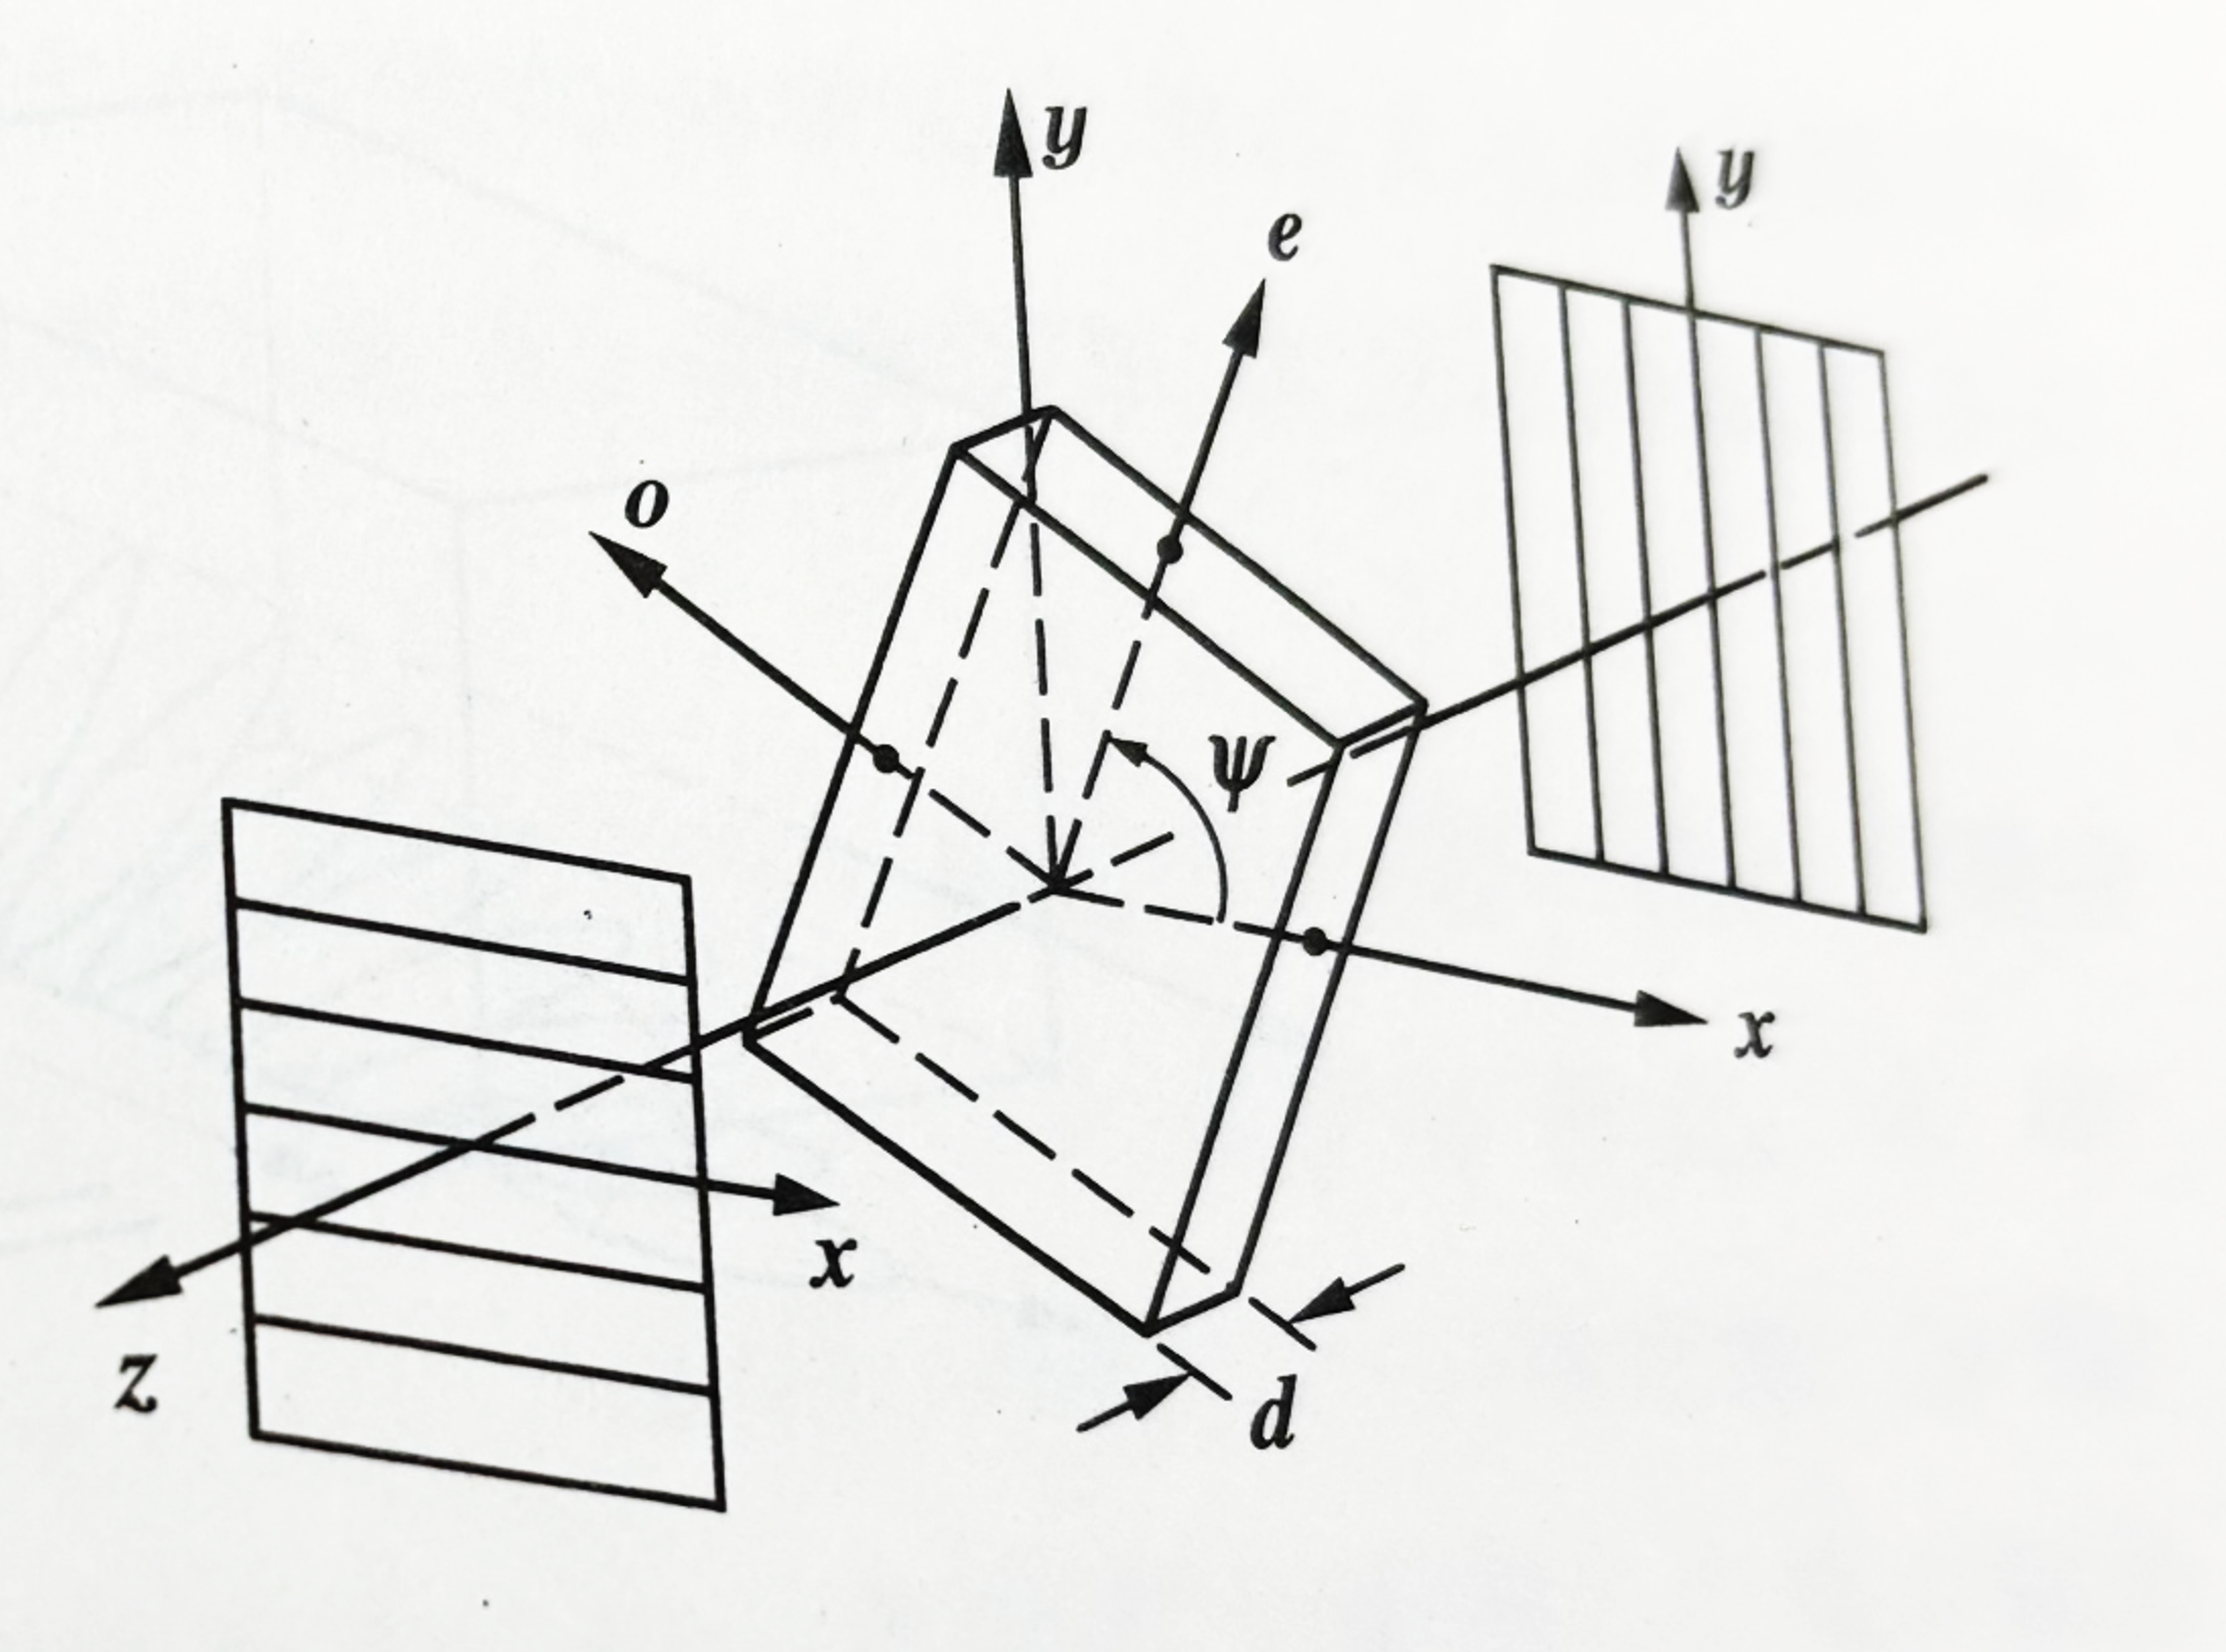
\includegraphics[width=0.92\linewidth]{appendix_2.png}
\caption{一軸位相差板をクロスニコル偏光板で挟んだ場合の光の伝搬.}
\label{fig:appendix_2}
\end{figure}

ここでは通常のJones計算の代表例として,透過軸が互いに直交する2枚の偏光板(クロスニコル)で
一軸の理想位相差板(リターダ)を挟んだ場合の出射光強度を導出する.
構成を図\ref{fig:appendix_2}に示す.

本文との整合のため,本節では偏光板を明示的なJones行列として挿入せず,
入射側偏光板は「入射偏光(透過後状態)の設定」,出射側偏光板(Analyzer)は「Analyzerの透過状態への射影」として扱う.
すなわち,入射側偏光板の透過状態を $\mathbf{o}_1$,解析器の透過状態を $\mathbf{o}_2$ とし,
層(ここでは位相差板)の作用素を $M$ とすると,透過振幅 $a$ と強度 $I_\perp$ は
\begin{equation}
a=\mathbf{o}_2^{\mathsf T} M\,\mathbf{o}_1\,E_0,
\qquad
I_\perp \propto |a|^2
\label{eq:main_form_amplitude}
\end{equation}
で与えられる.

以下,Jones基底を $(x,y)$ とし,入射側偏光板は $x$ 透過,Analyzerは $y$ 透過(クロスニコル条件)とする.
したがって許容状態は
\begin{equation}
\mathbf{o}_1=
\begin{pmatrix}
1\\
0
\end{pmatrix},
\qquad
\mathbf{o}_2=
\begin{pmatrix}
0\\
1
\end{pmatrix}
\label{eq:o1o2_xy}
\end{equation}
である(ここでは2次元表記を用いる).

位相差板は,主軸基底での位相差(retardation)を $\Gamma$ とし,
\eqref{eq:retarder} の $J(\Gamma)$ により表す.
主軸が入射偏光板の透過軸($x$)から角度 $\theta$ だけ回転しているとき,位相差板のJones行列は
\eqref{eq:retarder_rotated} により
\begin{equation}
M_{\mathrm{ret}}(\theta,\Gamma)=R(-\theta)\,J(\Gamma)\,R(\theta)
\label{eq:Mret_again}
\end{equation}
である.

入射光は入射偏光板を通過した $x$ 直線偏光(振幅 $E_0$)として与える:
\begin{equation}
\mathbf{j}_{\mathrm{in}}
=
E_0\,\mathbf{o}_1
=
\begin{pmatrix}
E_0\\
0
\end{pmatrix}.
\label{eq:jin_xpol}
\end{equation}
このとき,解析器透過成分の振幅は
\begin{equation}
a
=
\mathbf{o}_2^{\mathsf T} \,M_{\mathrm{ret}}(\theta,\Gamma)\,\mathbf{j}_{\mathrm{in}}
=
E_0\,\mathbf{o}_2^{\mathsf T} \,M_{\mathrm{ret}}(\theta,\Gamma)\,\mathbf{o}_1
\label{eq:a_def}
\end{equation}
で与えられる.すなわち本節は,明示的な偏光板行列を用いず
(入射側は初期条件,出射側は射影として)透過強度を求める計算例になっている.

\eqref{eq:Mret_again} を用いて $a$ を計算すると,
\begin{align}
\mathbf{o}_2^{\mathsf T}M_{\mathrm{ret}}(\theta,\Gamma)\mathbf{o}_1
&=
\begin{pmatrix}0&1\end{pmatrix}
R(-\theta)\,J(\Gamma)\,R(\theta)
\begin{pmatrix}1\\0\end{pmatrix}
\nonumber\\
&=
\frac{1}{2}\sin(2\theta)\Bigl(e^{+i\Gamma/2}-e^{-i\Gamma/2}\Bigr)
=
i\,\sin(2\theta)\,\sin\!\left(\frac{\Gamma}{2}\right),
\label{eq:a_over_E0}
\end{align}
(位相因子 $i$ は強度には寄与しない).
したがって
\begin{equation}
a
=
iE_0\,\sin(2\theta)\,\sin\!\left(\frac{\Gamma}{2}\right),
\label{eq:Ey_out}
\end{equation}
となり,透過強度は
\begin{equation}
I_{\perp}
\;\propto\;
|a|^2
=
|E_0|^2\,\sin^2(2\theta)\,\sin^2\!\left(\frac{\Gamma}{2}\right).
\label{eq:I_crossed_retarder}
\end{equation}
入射強度 $I_0\propto |E_0|^2$ を用いれば
\begin{equation}
\frac{I_{\perp}}{I_0}
=
\sin^2(2\theta)\,\sin^2\!\left(\frac{\Gamma}{2}\right)
\label{eq:Iratio_crossed_retarder}
\end{equation}
が得られる.これはクロスニコル間に挿入した位相差板の標準結果であり,
透過が(i)主軸方位 $\theta$ と(ii)位相差 $\Gamma$ の両方で制御されることを示す.

\subsection{式\eqref{eq:Iratio_crossed_retarder}に基づくIPSの暗状態・明状態の解釈}
\label{sec:IPS_dark_bright_from_crossed}

IPS(In-Plane Switching)では,電圧印加により液晶ディレクタ(有効光学軸)が基板面内で回転し,
光学軸方位角が $\phi(V)$ として変化する(面内回転が主効果)とみなせる.
正入射近傍では,液晶層は「一軸位相差板」として近似でき,
その有効位相差を $\Gamma(V)$,偏光板透過軸に対する主軸角を
\begin{equation}
\theta(V)=\phi(V)-\phi_{\mathrm{pol}}
\label{eq:theta_of_V}
\end{equation}
とおけば,クロスニコル構成における透過は
\begin{equation}
\frac{I_{\perp}(V)}{I_0}
=
\sin^2\!\bigl(2\theta(V)\bigr)\,
\sin^2\!\left(\frac{\Gamma(V)}{2}\right)
\label{eq:Iratio_IPS_simple}
\end{equation}
で表される.

\textbf{暗状態(Normally Black の基本像)}:
IPSの代表的な動作は「オフで暗,オンで明」である.
クロスニコル構成で $V=0$ のときディレクタが偏光板透過軸に整列していれば
\begin{equation}
\theta(0)\approx 0 \quad (\text{または } \pi/2)
\end{equation}
となり,
\begin{equation}
\sin^2\!\bigl(2\theta(0)\bigr)\approx 0
\quad\Rightarrow\quad
I_{\perp}(0)\approx 0
\label{eq:dark_condition}
\end{equation}
が得られる.すなわち暗状態は主に「面内方位がクロス条件を満たす」ことにより実現される.

\textbf{明状態(オンで透過を最大化)}:
電圧を印加してディレクタが面内で回転し,
\begin{equation}
\theta(V)\to \frac{\pi}{4}
\label{eq:bright_angle}
\end{equation}
に近づくと,$\sin^2(2\theta)$ が最大(=1)となり,
\begin{equation}
\frac{I_{\perp}(V)}{I_0}\approx \sin^2\!\left(\frac{\Gamma(V)}{2}\right)
\label{eq:bright_limited_by_Gamma}
\end{equation}
まで透過が増大する.従って明状態の上限は位相差 $\Gamma(V)$ により規定される.
特に
\begin{equation}
\Gamma(V)\approx \pi \quad (\text{半波条件})
\end{equation}
が満たされる波長では $\sin^2(\Gamma/2)\approx 1$ となり高透過が得られる.
一方,$\Gamma$ は波長依存性(分散)と厚み・複屈折に依存するため,
実際のIPSでは補償膜等により視野角・波長での最適化が行われる.

以上より,式\eqref{eq:Iratio_IPS_simple}の観点からは,
IPSの暗・明状態は次の二つの因子に分離して理解できる:
\begin{enumerate}
\item 面内回転による主軸角 $\theta(V)$ の制御(幾何学因子 $\sin^2(2\theta)$)
\item 層の有効位相差 $\Gamma(V)$ の制御(位相因子 $\sin^2(\Gamma/2)$)
\end{enumerate}
IPSでは主として (1) が変調の主因であり,
(2) は波長・視野角・材料定数・厚みで決まる設計パラメータとして透過上限や色特性を支配する,
という整理が得られる.

